\subsection{Functional Reactive Programming}
\label{sec:step2_frp}
TODO: rewrite this section because now we don't have a naive beginnings section anymore

As shown in the first step, the need to handle $\Delta t$ explicitly can be quite messy, is inelegant and a potential source of errors, also the explicit handling of the state of an agent and its behavioural function is not very modular. We can solve both these weaknesses by switching to the Functional Reactive Programming paradigm, because it allows to express systems with discrete and continuous time-semantics.

In this step we are focusing on Arrowized FRP \cite{hughes_generalising_2000} using the library Yampa \cite{hudak_arrows_2003}. In it, time is handled implicitly, meaning it cannot be messed with, which is achieved by building the whole system on the concept of signal functions (SF). An SF can be understood as a process over time and is technically a continuation which allows to capture state using closures. Both these fundamental features allow us to tackle the weaknesses of our first step and push our approach further towards a truly functional approach by using declarative FRP idioms encoding a stateless approach.

\subsubsection{Implementation}
We start by defining the SIR states and agent to be an SF which receives the SIR states of all agents as input and outputs the SIR state of the agent:

\begin{HaskellCode}
data SIRState = Susceptible | Infected | Recovered

type SIRAgent = SF [SIRState] SIRState 
\end{HaskellCode}

Now we can define the behaviour of an agent to be the following:

\begin{HaskellCode}
sirAgent :: RandomGen g => g -> SIRState -> SIRAgent
sirAgent g Susceptible = susceptibleAgent g
sirAgent g Infected    = infectedAgent g
sirAgent _ Recovered   = recoveredAgent
\end{HaskellCode}

Depending on the initial state we return the corresponding behaviour. Most notably is the difference that we are now passing a random-number generator instead of running in the Random Monad because signal functions as implemented in Yampa are not capable of being monadic. We see that the recovered agent ignores the random-number generator which is in accordance with the implementation in the previous step where it acts as a sink which returns constantly the same state:

These agents do nothing because this state is a consuming state from which there is no escape: recovered agents stay immune and can not get infected again in this model. 

\begin{HaskellCode}
recoveredAgent :: SIRAgent
recoveredAgent = arr (const Recovered)
\end{HaskellCode}

An agent gets fed the states of all agents in the system from the previous time-step so it can draw random contacts - this is one, very naive way of implementing the interactions between agents.

From our implementation it becomes apparent that only the behaviour of a susceptible agent involves randomness and that a recovered agent is simply a sink - it does nothing and stays constant.

Lets look how we can implement the behaviour of a susceptible agent. It simply makes contact on average with a number of other agents and gets infected with a given probability if an agent it has contact with is infected. Here it becomes apparent that we implicitly assume that the simulation is stepped with a $\Delta t = 1.0$. If we would use a different $\Delta t$ then we need to adjust the contact rate accordingly because it is defined \textit{per time-unit}. This would amount to multiplying with the $\Delta t$ which in combination with the discretisation using \textit{floor} would lead to too few contacts being made, ultimately resulting in completely wrong dynamics.

When an event occurs we can change the behaviour of an agent using the Yampa combinator \textit{switch}, which is much more elegant and expressive than the initial approach as it makes the change of behaviour at the occurrence of an event explicit. Thus a susceptible agent behaves as susceptible until it becomes infected. Upon infection an \textit{Event} is returned which results in switching into the \textit{infectedAgent} SF, which causes the agent to behave as an infected agent from that moment on. Instead of randomly drawing the number of contacts to make, we now follow a fundamentally different approach by using Yampas \textit{occasionally} function. This requires us to carefully select the right $\Delta t$ for sampling the system as will be shown in results. 

A susceptible agent makes contact \textit{on average} with $\beta$ other random agents. For every \textit{infected} agent it gets into contact with, it becomes infected with a probability of $\gamma$. If an infection happens, it makes the transition to the \textit{Infected} state.

%\begin{samepage}
\begin{HaskellCode}
susceptibleAgent :: RandomGen g => g -> SIRAgent
susceptibleAgent g = 
    switch (susceptible g) (const (infectedAgent g))
  where
    susceptible :: RandomGen g 
      => g -> SF [SIRState] (SIRState, Event ())
    susceptible g = proc as -> do
      makeContact <- occasionally g (1 / contactRate) () -< ()
      if isEvent makeContact
        then (do
          a <- drawRandomElemSF g -< as
          case a of
            Infected -> do
              i <- randomBoolSF g infectivity -< ()
              if i
                then returnA -< (Infected, Event ())
                else returnA -< (Susceptible, NoEvent)
             _       -> returnA -< (Susceptible, NoEvent))
        else returnA -< (Susceptible, NoEvent)
\end{HaskellCode}
%\end{samepage}

We deal with randomness differently now and implement signal functions built on the \textit{noiseR} function provided by Yampa. This is an example for the stream character and statefulness of a signal function as it needs to keep track of the changed random-number generator internally through the use of continuations and closures. Here we provide the implementation of \textit{randomBoolSF}. \textit{drawRandomElemSF} works similar but takes a list as input and returns a randomly chosen element from it:

\begin{HaskellCode}
randomBoolSF :: RandomGen g => g -> Double -> SF () Bool
randomBoolSF g p = proc _ -> do
  r <- noiseR ((0, 1) :: (Double, Double)) g -< ()
  returnA -< (r <= p)
\end{HaskellCode}

The infected agent behaves as infected until it recovers, on average after the illness duration, after which it behaves as a recovered agent by switching into \textit{recoveredAgent}. As in the case of the susceptible agent, we use the \textit{occasionally} function to generate the event when the agent recovers. Note that the infected agent ignores the states of the other agents as its behaviour is completely independent of them.

An infected agent recovers \textit{on average} after $\delta$ time units. This is implemented by drawing the duration from an exponential distribution \cite{borshchev_system_2004} with $\lambda = \frac{1}{\delta}$ and making the transition to the \textit{Recovered} state after this duration.

\begin{HaskellCode}
infectedAgent :: RandomGen g => g -> SIRAgent
infectedAgent g = switch infected (const recoveredAgent)
  where
    infected :: SF [SIRState] (SIRState, Event ())
    infected = proc _ -> do
      recEvt <- occasionally g illnessDuration () -< ()
      let a = event Infected (const Recovered) recEvt
      returnA -< (a, recEvt)
\end{HaskellCode}

Running and stepping the simulation works now a bit differently, using Yampas function \textit{embed}:

\begin{HaskellCode}
runSimulation :: RandomGen g 
  => g -> Time -> DTime -> [SIRState] -> [[SIRState]]
runSimulation g t dt as 
    = embed (stepSimulation sfs as) ((), dts)
  where
    steps     = floor (t / dt)
    dts       = replicate steps (dt, Nothing)
    n         = length as
    (rngs, _) = rngSplits g n [] -- unique rngs for each agent
    sfs       = zipWith sirAgent rngs as
\end{HaskellCode}

What we need to implement next is a closed feedback-loop - the heart of every agent-based simulation. Fortunately, \cite{nilsson_functional_2002, courtney_yampa_2003} discusses implementing this in Yampa. The function \textit{stepSimulation} is an implementation of such a closed feedback-loop. It takes the current signal functions and states of all agents, runs them all in parallel and returns this step's new agent states. Note the use of \textit{notYet} which is required because in Yampa switching occurs immediately at $t = 0$. If we don't delay the switching at $t = 0$ until the next step, we would enter an infinite switching loop - \textit{notYet} simply delays the first switching until the next time-step.

\begin{HaskellCode}
stepSimulation :: [SIRAgent] -> [SIRState] -> SF () [SIRState]
stepSimulation sfs as =
    dpSwitch
      -- feeding the agent states to each SF
      (\_ sfs' -> (map (\sf -> (as, sf)) sfs'))
      -- the signal functions
      sfs
      -- switching event, ignored at t = 0         
      (switchingEvt >>> notYet)
      -- recursively switch back into stepSimulation         
      stepSimulation                            
  where
    switchingEvt :: SF ((), [SIRState]) (Event [SIRState])
    switchingEvt = arr (\ (_, newAs) -> Event newAs)
\end{HaskellCode}

Yampa provides the \textit{dpSwitch} combinator for running signal functions in parallel, which has the following type-signature:

\begin{HaskellCode}
dpSwitch :: Functor col
         -- routing function
         => (forall sf. a -> col sf -> col (b, sf))
         -- SF collection
         -> col (SF b c)
         -- SF generating switching event     
         -> SF (a, col c) (Event d)
         -- continuation to invoke upon event           
         -> (col (SF b c) -> d -> SF a (col c))
         -> SF a (col c)
\end{HaskellCode}

Its first argument is the pairing-function which pairs up the input to the signal functions - it has to preserve the structure of the signal function collection. The second argument is the collection of signal functions to run. The third argument is a signal function generating the switching event. The last argument is a function which generates the continuation after the switching event has occurred. \textit{dpSwitch} returns a new signal function which runs all the signal functions in parallel and switches into the continuation when the switching event occurs. The d in \textit{dpSwitch} stands for decoupled which guarantees that it delays the switching until the next time-step: the function into which we switch is only applied in the next step, which prevents an infinite loop if we switch into a recursive continuation.

Conceptually, \textit{dpSwitch} allows us to recursively switch back into the \textit{stepSimulation} with the continuations and new states of all the agents after they were run in parallel. 

\subsubsection{Results}
The dynamics generated by this step can be seen in Figure \ref{fig:sir_abs_dynamics_frp}. 

\begin{figure}
\begin{center}
	\begin{tabular}{c c}
		\begin{subfigure}[b]{0.22\textwidth}
			\centering
			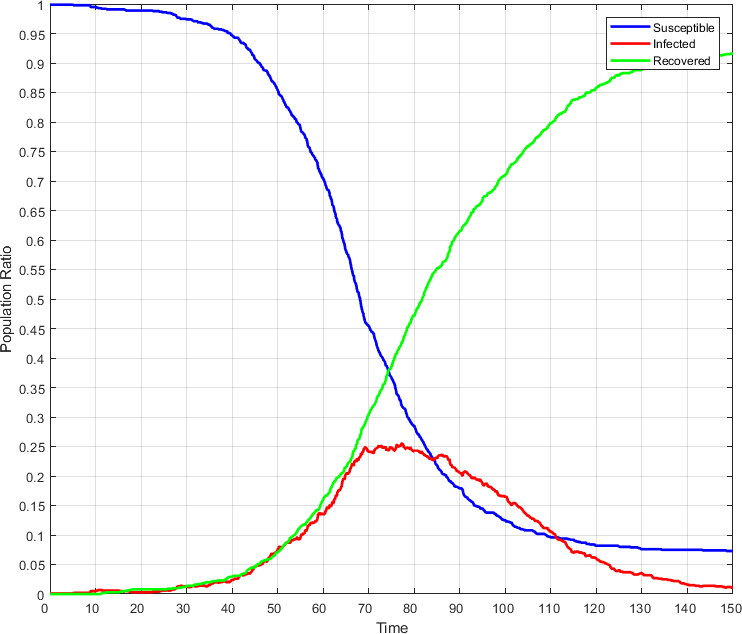
\includegraphics[width=1\textwidth, angle=0]{./fig/step2_yampa/SIR_1000agents_150t_01dt.png}
			\caption{$\Delta t = 0.1$}
			\label{fig:sir_abs_approximating_01dt_1000agents}
		\end{subfigure}
		
		&
    	
		\begin{subfigure}[b]{0.22\textwidth}
			\centering
			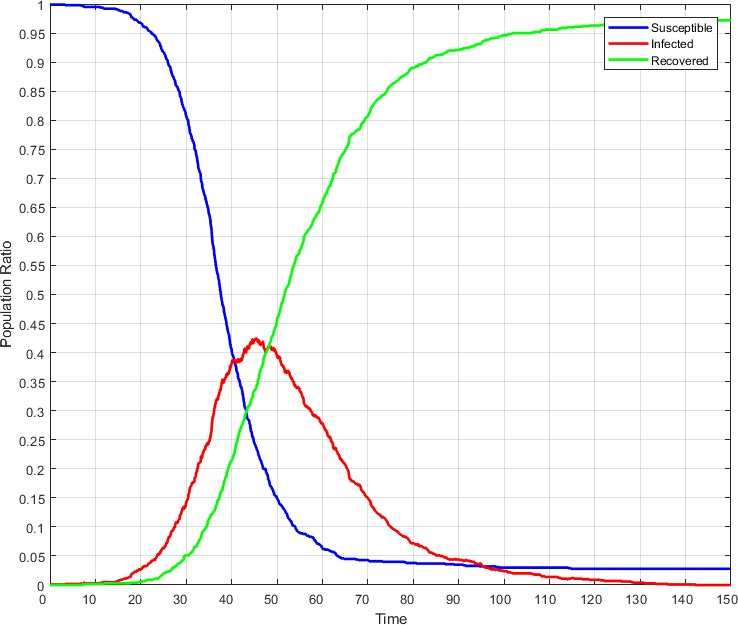
\includegraphics[width=1\textwidth, angle=0]{./fig/step2_yampa/SIR_1000agents_150t_001dt.png}
			\caption{$\Delta t = 0.01$}
			\label{fig:sir_abs_approximating_001dt_1000agents}
		\end{subfigure}
	\end{tabular}
	
	\caption{FRP simulation of agent-based SIR showing the influence of different $\Delta t$. Population size of 1,000 with contact rate $\beta = \frac{1}{5}$, infection probability $\gamma = 0.05$, illness duration $\delta = 15$ with initially 1 infected agent. Simulation run for 150 time-steps with respective $\Delta t$.} 
	\label{fig:sir_abs_dynamics_frp}
\end{center}
\end{figure}

In this step we followed the FRP approach which is fundamentally different from the previous step in Section \ref{sec:naive_beginnigs} because in FRP we assume a continuous flow of time as opposed to discrete time-steps of $\Delta t = 1.0$ previously. This means that we need to select a \textit{correct} $\Delta t$ otherwise we would end up with wrong dynamics. The selection of a correct $\Delta t$ depends in our case on \textit{occasionally} in the \textit{susceptible} behaviour, which randomly generates an event on average with \textit{contact rate} following the exponential distribution. To arrive at the correct dynamics, this requires us to sample \textit{occasionally}, and thus the whole system, with small enough $\Delta t$ which matches the frequency of events generated by \textit{contact rate}. If we choose a too large $\Delta t$, we loose events which will result in wrong dynamics as can be seen in Figure \ref{fig:sir_abs_approximating_01dt_1000agents}. This issue is known as under-sampling and is described in Figure \ref{fig:sampling_issue}.

\begin{figure}
\begin{center}
	\begin{tabular}{c}
		\begin{subfigure}[b]{0.3\textwidth}
			\centering
			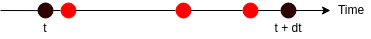
\includegraphics[width=1\textwidth, angle=0]{./fig/diagrams/Undersampling.png}
			\caption{Under-sampling}
			\label{fig:undersampling}
		\end{subfigure}
		
		\\
		
		\begin{subfigure}[b]{0.3\textwidth}
			\centering
			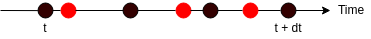
\includegraphics[width=1\textwidth, angle=0]{./fig/diagrams/Supersampling.png}
			\caption{Super-sampling}
			\label{fig:supersampling}
		\end{subfigure}
	\end{tabular}
	
	\caption{A visual explanation of under-sampling and super-sampling. The black dots represent the time-steps of the simulation. The red dots represent virtual events which occur at specific points in continuous time. In the case of under-sampling, 3 events occur in between the two time steps but \textit{occasionally} only captures the first one. By increasing the sampling frequency either through a smaller $\Delta t$ or super-sampling all 3 events can be captured.} 
	\label{fig:sampling_issue}
\end{center}
\end{figure}

For tackling this issue we have two options. The first one is to use a smaller $\Delta t$ as can be seen \ref{fig:sir_abs_approximating_001dt_1000agents}, which results in the whole system being sampled more often, thus reducing performance. The other option is to implement super-sampling and apply it to \textit{occasionally} which would allow us to run the whole simulation with $\Delta t = 1.0$ and only sample the \textit{occasionally} function with a much higher frequency.

An approach to super-sampling would be to introduce a new combinator to Yampa which allows us to super-sample other signal functions. 

\begin{HaskellCode}
superSampling :: Int -> SF a b -> SF a [b]
\end{HaskellCode}

It evaluates the \textit{SF} argument for \textit{n} times, each with $\Delta t = \frac{\Delta t}{n}$ and the same input argument \textit{a} for all \textit{n} evaluations. At time 0 no super-sampling is performed and just a single output of the \textit{SF} argument is calculated. A list of \textit{b} is returned with length of \textit{n} containing the result of the \textit{n} evaluations of the \textit{SF} argument. If 0 or less super samples are requested exactly one is calculated. We could then wrap the occasionally function which would then generate a list of events. We have investigated super-sampling more in-depth but have to omit this due to lack of space.

\subsubsection{Discussion}
We can conclude that it already introduced most of the fundamental concepts of ABS
\begin{itemize}
	\item Time - the simulation occurs over virtual time which is modelled explicitly divided into \textit{fixed} $\Delta t$ where at each step all agents are executed.
	\item Agents - we implement each agent as an individual, with the behaviour depending on its state.
	\item Feedback - the output state of the agent in the current time-step $t$ is the input state for the next time-step $t + \Delta t$.
	\item Environment - as environment we implicitly assume a fully-connected network (complete graph) where every agent 'knows' every other agent, including itself and thus can make contact with all of them.
	\item Stochasticity - it is an inherently stochastic simulation, which is indicated by the Random Monad type and the usage of \textit{randomBoolM} and \textit{randomExpM}.
	\item Deterministic - repeated runs with the same initial random-number generator result in same dynamics. This may not come as a surprise but in Haskell we can guarantee that property statically already at compile time because our simulation runs in the Random Monad and \textit{not} in the IO Monad. This guarantees that no external, uncontrollable sources of non-determinism can interfere with the simulation.
\end{itemize}

By using FRP in the instance of Yampa we made an improvement in clarity, expressivity and robustness of our implementation. State is now implicitly encoded, depending on which signal function is active. Also by using explicit time-semantics with \textit{occasionally} we can achieve extremely fine grained stochastics. Compared to drawing a random number of events we create only a single event or none at all. This requires to sample the system with a much smaller $\Delta t$ than in the previous step: we are treating it as a truly continuous agent-based system.

A very severe problem, very hard to find with testing but detectable with in-depth validation analysis, is the fact that in the \textit{susceptible} agent the same random-number generator is used in \textit{occasionally}, \textit{drawRandomElemSF} and \textit{randomBoolSF}. This means that all three stochastic functions, which should be independent from each other, are inherently correlated. This is something one wants to prevent under all circumstances in a simulation, as it can invalidate the dynamics on a very subtle level, and indeed we have tested the influence of the correlation in this example and it has an impact. We left this severe bug in for explanatory reasons, as it shows an example where functional programming actually encourages very subtle bugs if one is not careful. A possible solution would be to simply split the initial random-number generator in \textit{sirAgent} three times (using one of the splited generators for the next split) and pass three random-number generators to \textit{susceptible}. Note that this is not an issue in Sections \ref{sec:naive_beginnigs} and \ref{sec:generalising_msfs} as we are using the Random Monad, which never uses the same random-number generator twice thus resulting in guaranteed uncorrelated stochastics.

So far we have an acceptable implementation of an agent-based SIR approach. What we are lacking at the moment is a general treatment of an environment. To conveniently introduce it we want to make use of monads which is not possible using Yampa. In the next step we make the transition to Monadic Stream Functions as introduced in Dunai \cite{perez_functional_2016} which allows FRP within a monadic context.